\lecture[1]{Remotely Connected Electric Field\\ Generator}{lecture-text}

\subtitle{for Particle Separation in a Fluid}

\date{27 April 2016}


\begin{document}

\begin{frame}
  \maketitle
\end{frame}

% justin
\section{Dielectrophoresis}

% justin
\begin{frame}{Dielectrophoresis (DEP)}
  \begin{multicols}{2}

  \begin{block}{}
  \begin{itemize}
  \item A dielectric particle in a non uniform 
  electric field experiences a force
  \item Different potential fields and frequencies 
  has an effect on the net force
  \item First studied in 1950s by Herbert Pohl
  \end{itemize}
  \end{block}

  \newpage

  \begin{center}
  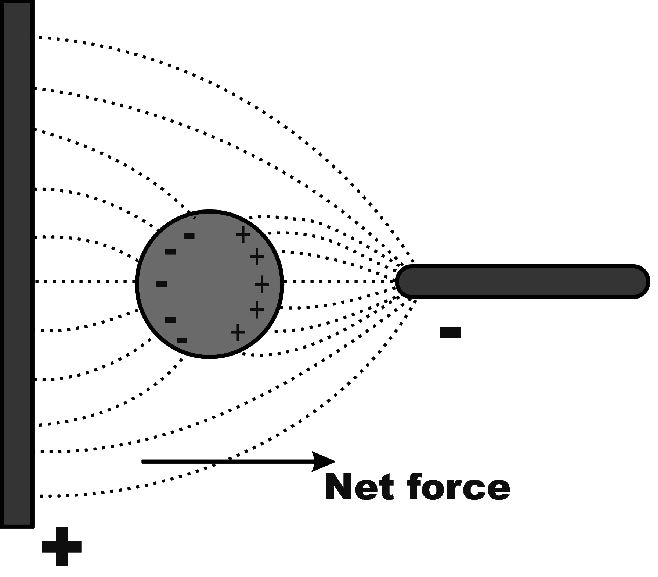
\includegraphics[width=0.5\textwidth,keepaspectratio]{dep.pdf}
  \end{center}

  \end{multicols}
\end{frame}

% justin
\begin{frame}{Real World Application}
  \begin{block}{Dielectrophoresis}
  \begin{itemize}
    \item Recently revived due to the ability to
  manipulate micro-particles and cells. 
    \item Potential to separate particles in spinal fluid
    \item Act as filter
    \item Research in separating cancerous cells from healthy cells
    \item Separate platelets from whole blood
    \item Separate red and white blood cells
    \item Separate Strains of bacteria and viruses from living cells
  \end{itemize}
  \end{block}
\end{frame}

% tim
\section{Project Overview}

\begin{frame}{Project Description}
\begin{block}{}
  \begin{itemize}
    \item A system to aid in of DEP research
    \item Allow for quicker setup times
    \item Control Voltage and Frequency via the web
      \begin{itemize}
        \item 1 to 60 VPP
        \item 10k to 1Mhz
      \end{itemize}
    \item Hold output for long time periods
    \item Small Form Factor
    \item Easy to use
    \item Plug and play
  \end{itemize}
\end{block}
\end{frame}

% talk about what motivated the choise of a raspberry pi
\begin{frame}{Project Structure}
  \begin{multicols}{2}
  \begin{itemize}
    \item Raspberry Pi
    \item Web Interface
    \item Web Server
    \item Frequency Control Solution
    \item Voltage Control Solution
  \end{itemize}

  \newpage

  %\begin{center}
  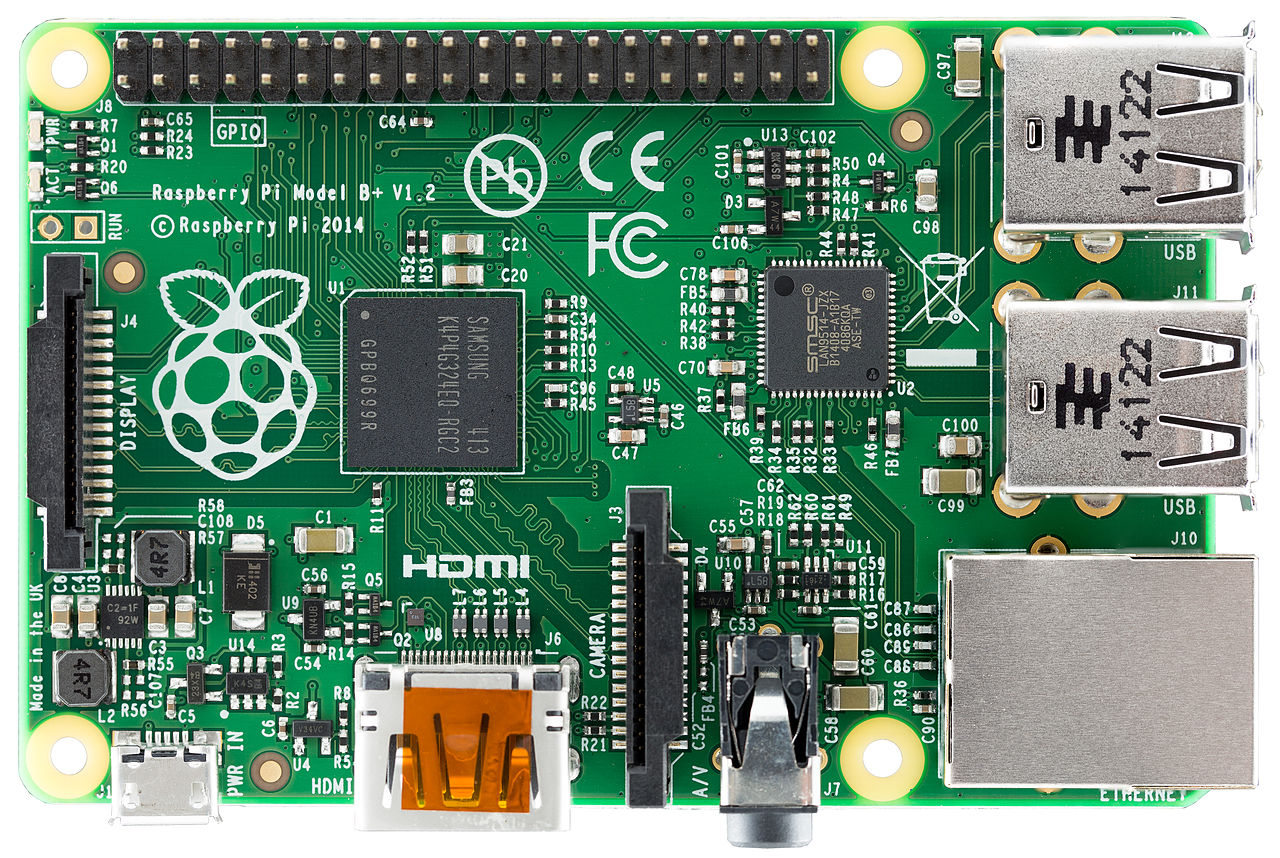
\includegraphics[width=0.5\textwidth,keepaspectratio]{rpi_real.png}
  %\end{center}

  \end{multicols}
\end{frame}

\section{Initial Implementation}

\subsection{Design}

\begin{frame}{Initial Implementation}
  \begin{block}{}
  \begin{itemize}
    \item Raspberry Pi 
      \begin{itemize}
        \item Host web server
        \item Remote manipulation of circuit output
        \item Web interface can provide additional functionality
        \item GPIO pins input to circuit
      \end{itemize}
    \item Circuit Output
      \begin{itemize}
        \item Frequency generated by GPIO pin 
        \item GPIO waveform integrated to get sine wave
        \item Sine wave amplified to form output
      \end{itemize}
    \end{itemize}
  \end{block}

  \begin{center}
  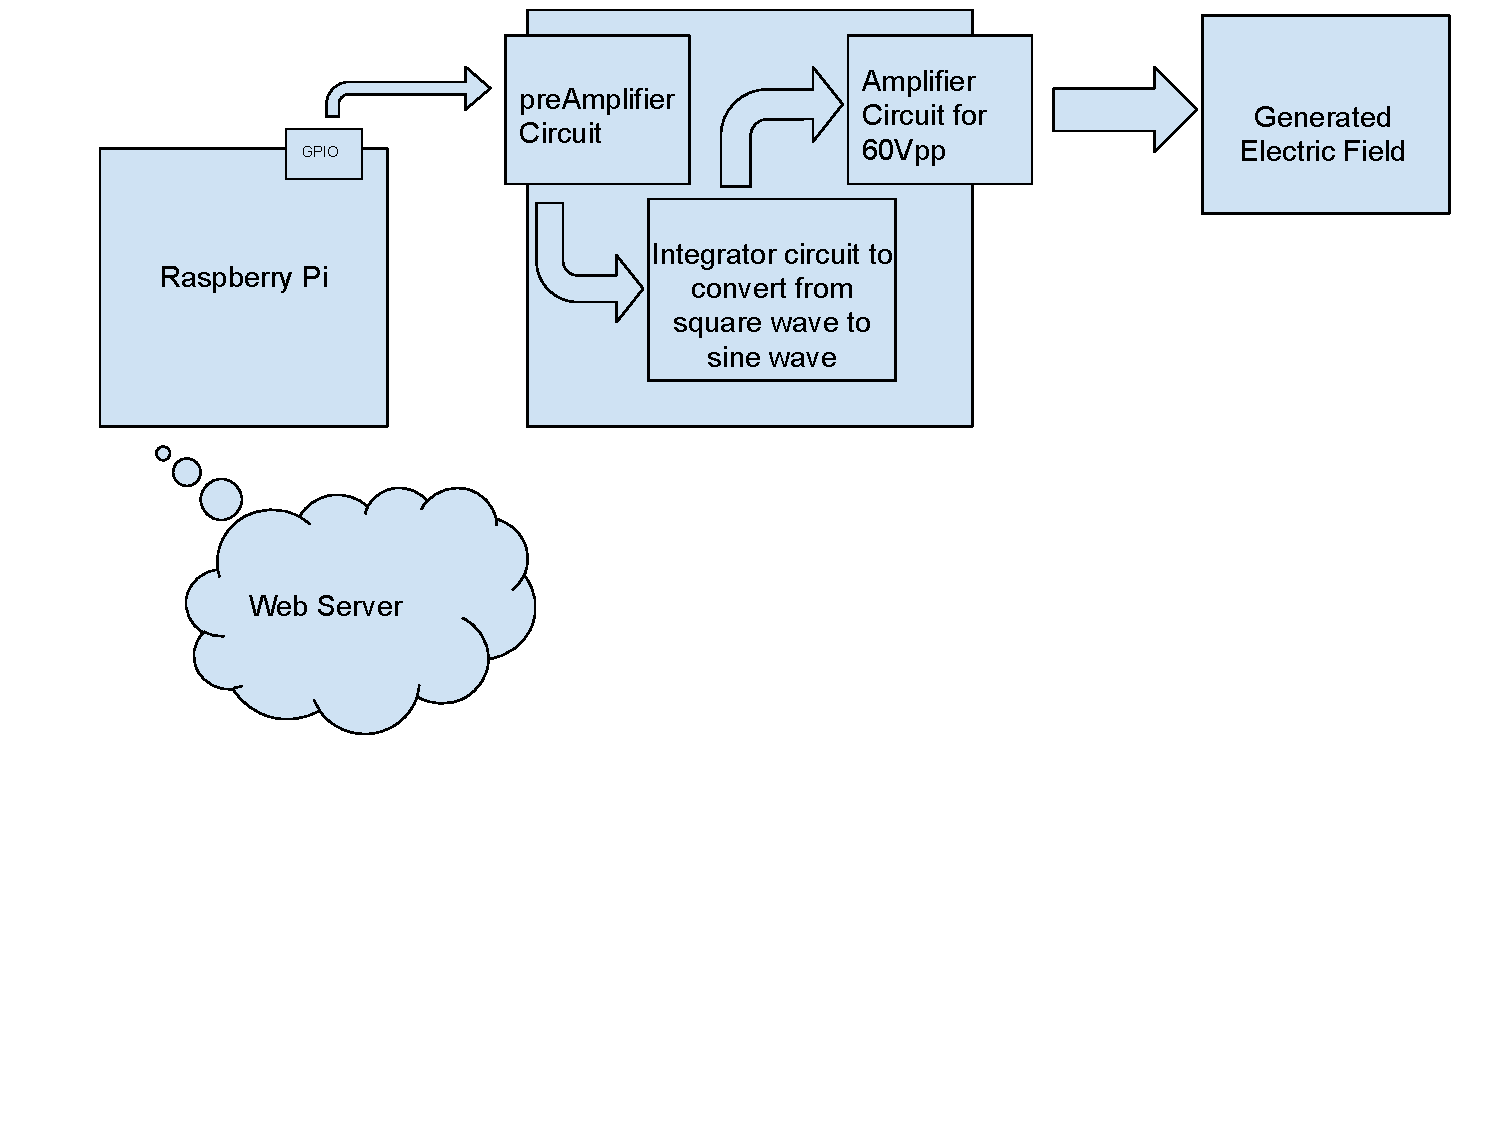
\includegraphics[width=0.8\textwidth,keepaspectratio]{flowchart_version_1.pdf}
  \end{center}
\end{frame}

\subsection{Problems}

\begin{frame}{Concerns}
  \begin{block}{}
  \begin{itemize}
    \item Raspberry Pi 
      \begin{itemize}
        \item Complexity of programming
        \item GPIO pins may only be turned on and off
        \item On-off mechanism must be used to generate waveform
        % pi cannot handle alot of output current
        \item Current load
      \end{itemize}
    \item Circuit Output
      \begin{itemize}
        \item Complexity of construction
        \item No guarantees about cleanliness of GPIO pin waveform 
        \item High risk of failure
      \end{itemize}
    \end{itemize}
  \end{block}

\end{frame}

% end of first semester
\section{Intermediate Implementation 1}

\subsection{Design}

\begin{frame}{Minigen Function Generator}
  %\begin{multicols}{2}
  
  \begin{itemize}
    \item SPI communications
    \item Small form factor
    \item Output programmable frequency 
    \item Produces 1 Khz to 4 Mhz waveforms
  \end{itemize}

  %\newpage

  \begin{center}
  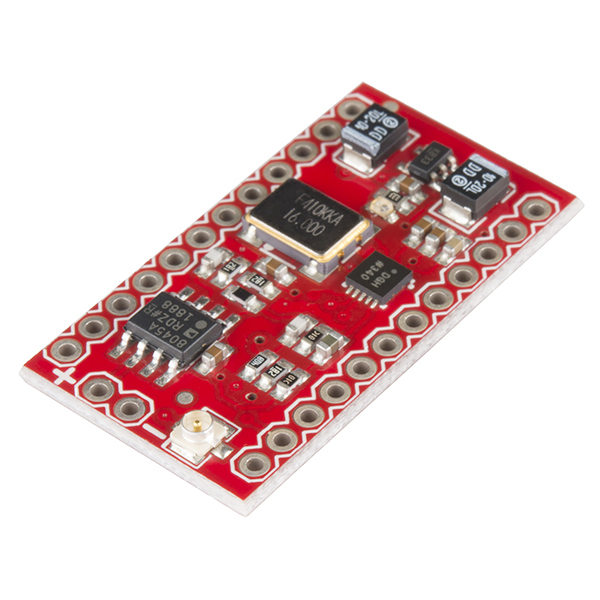
\includegraphics[width=0.8\textwidth,keepaspectratio]{minigen_real.png}
  \end{center}

  %\end{multicols}

\end{frame}

\begin{frame}{Intermediate Design}
  \begin{block}{}
  \begin{itemize}
    \item Raspberry Pi controls Integrated circuit components
    \item Minigen used to produce frequency
    \item Digital Potentiometers
      \begin{itemize}
      \item SPI communications
      \item Vary resistance to control amplifier
      \end{itemize}
    \item Amplifier controls voltage output from circuit
  \end{itemize}
  \end{block}
\end{frame}

\subsection{Implementation and Problems}

\begin{frame}{Digital Potentiometer Amplifier Circuit }
  \begin{block}{Properties}
  \begin{itemize}
    \item Utilizes digital potentiometer as feedback resistor
  \end{itemize}

  % formula
  \begin{center}
    $V_{out} = \frac{-R_F}{R_{IN}} * Minigen_{SIGNAL}$
  \end{center}
  \end{block}

  \begin{center}
  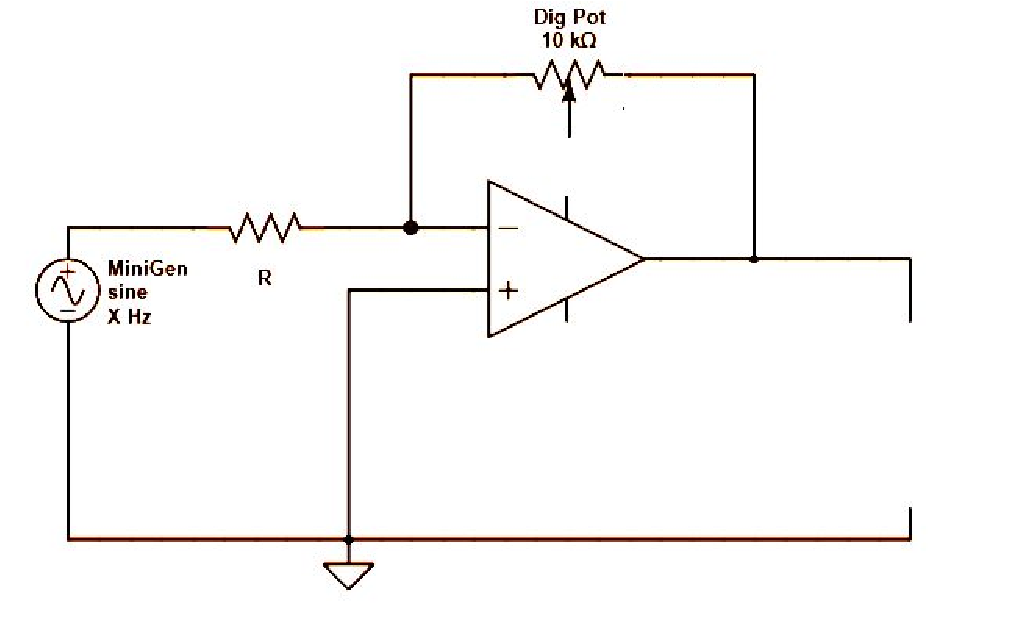
\includegraphics[width=0.5\textwidth,keepaspectratio]{digital_pot_amplifier.pdf}
  \end{center}

  \begin{block}{Problems}
    \begin{itemize}
      \item Distortion of signal
      \item Resistance drops with AC signal
    \end{itemize}    
  \end{block}
\end{frame}

\begin{frame}{MOSFET Amplifier}
  \begin{block}{Properties}
  \begin{itemize}
    \item Utilizes digital pot in a different way
    \item Amplification utilizes transistor
  \end{itemize}
  \end{block}

  \begin{multicols}{2}

  \begin{center}
  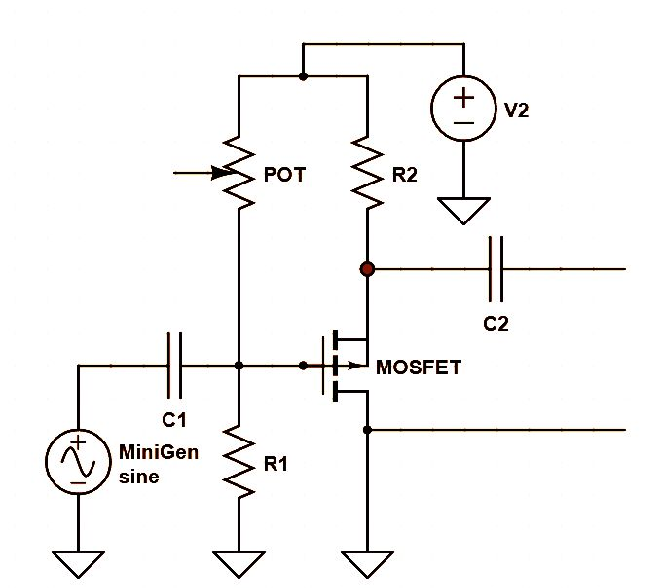
\includegraphics[width=0.5\textwidth,keepaspectratio]{mosfet_amplifier.pdf}
  \end{center}

  \newpage

  %\begin{block}{Problems}
    \begin{itemize}
      \item Distortion of signal remains
      \item Concluded digital potentiometer is source of problem
    \end{itemize}    
  %\end{block}

  \end{multicols}
\end{frame}

% \begin{frame}{Problems and Setbacks}
%   \begin{itemize}
%     \item MOSFET Amplifier
%       \begin{itemize}
%       \item Unable to produce clean waveform
%       \end{itemize}
%     \item Digital Potentiometer
%       \begin{itemize}
%       \item Resistance drops with AC signal
%       \item Distorted waveforms
%       \begin{itemize}
%     % discuss these things later
%     %\item Op Amps
%     %\item Slew Rates
%     %\item Gain Bandwidth
%     %\item Minigen
%     %\item B23 Bug
%   \end{itemize}
% \end{frame}

% beginning of second semester to middle of second semester
\section{Intermediate Implementation 2}

\subsection{Design}

\begin{frame}{Redesign Amplifier}
  \begin{block}{Idea Overview}
  \begin{itemize}
    \item Previous problems stem from voltage modification solutions
    \item Solution: Use integrated circuit component to modify voltage
  \end{itemize}
  \end{block}

  \begin{block}{Amplifier Properties}
  \begin{itemize}
    \item Three stages of amplification
    \item One PGA and two stages with constant gain
      \begin{itemize}
        \item $20V_{pp}$ per stage
        \item Summing amplifier sums stages
        \item PGA achieves 8 steps within one stage
        \item Switches increase output by $20V_{pp}$
      \end{itemize}
    \item Use transistors as switches flipped using GPIO pins
  \end{itemize}
  \end{block}

\end{frame}

\begin{frame}{Configuration}
  \begin{block}{Programmable Gain Amplifier(PGA)}
  \begin{itemize}
    \item Three pins encode gain
    \item 8 Gain Options from 0 to 7
  \end{itemize}
  \end{block}

%  \begin{multicols}{2}

  % \begin{itemize}
  %   \item Raspberry Pi connected to components
  %   \item Output of Minigen goes to input of PGA
  %   \item All three stages input to summing amplifier
  % \end{itemize}

 % \newpage

  \begin{center}
  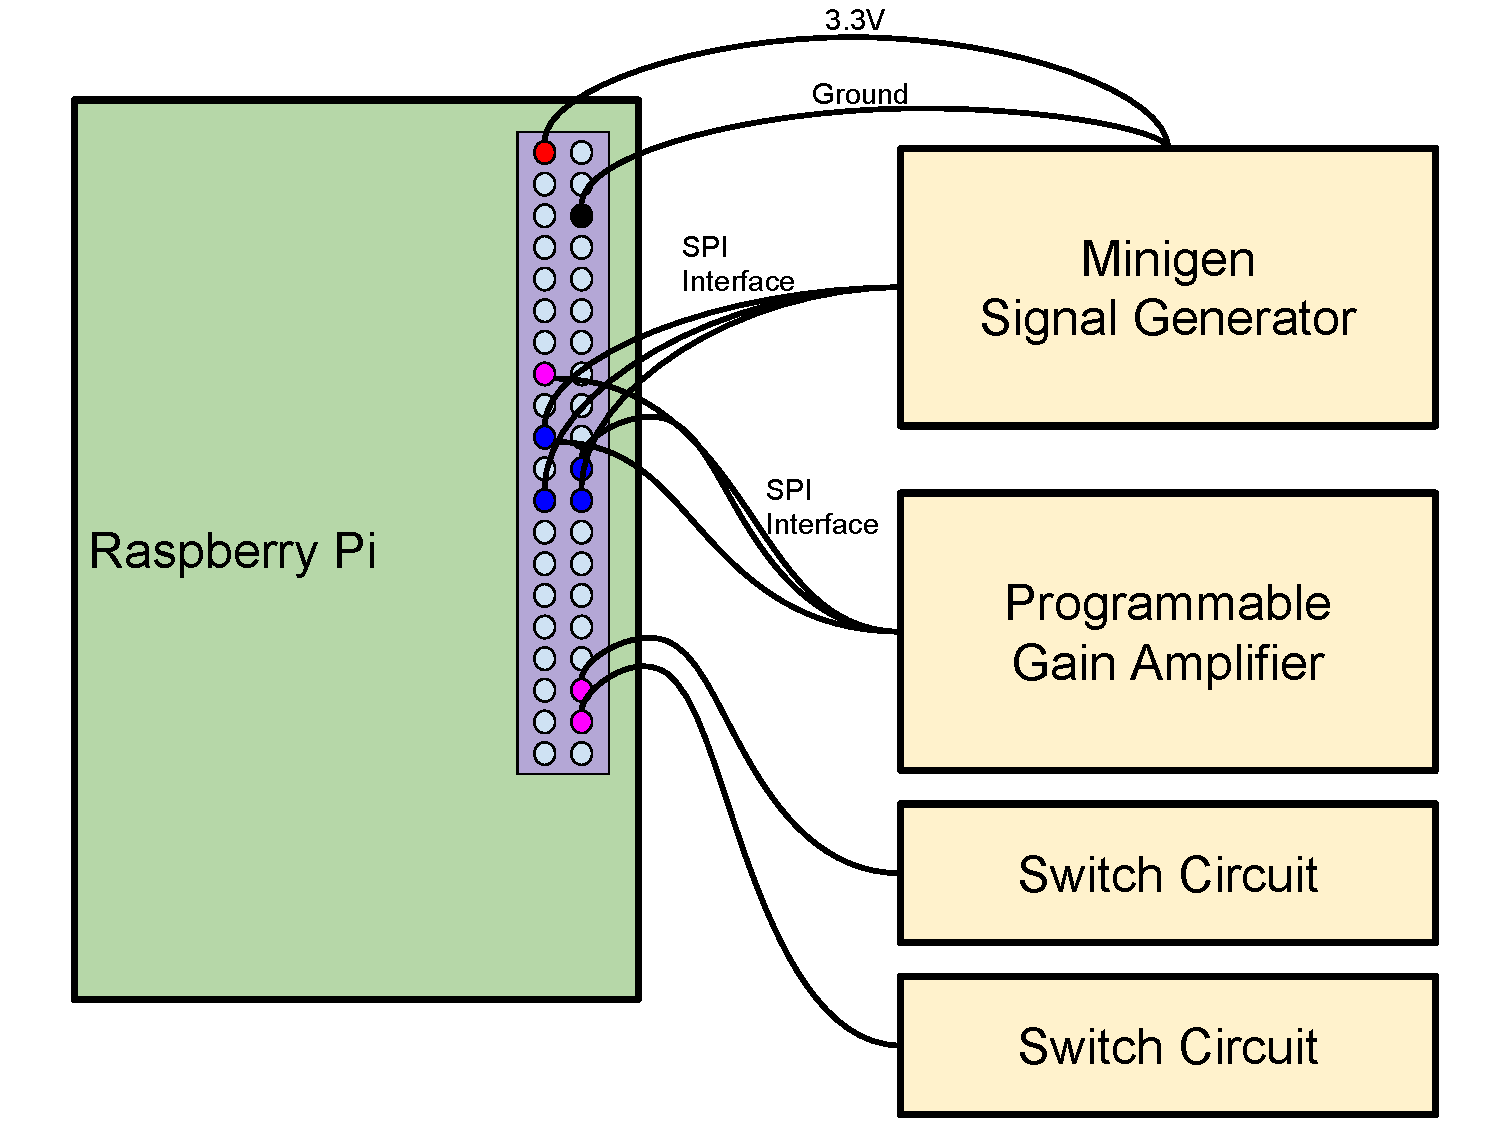
\includegraphics[width=0.8\textwidth,keepaspectratio]{pi_connection.pdf}
  \end{center}

  %\end{multicols}
\end{frame}

\subsection{Implementation}

\begin{frame}{SSR Circuit Implementation}
  \begin{center}
  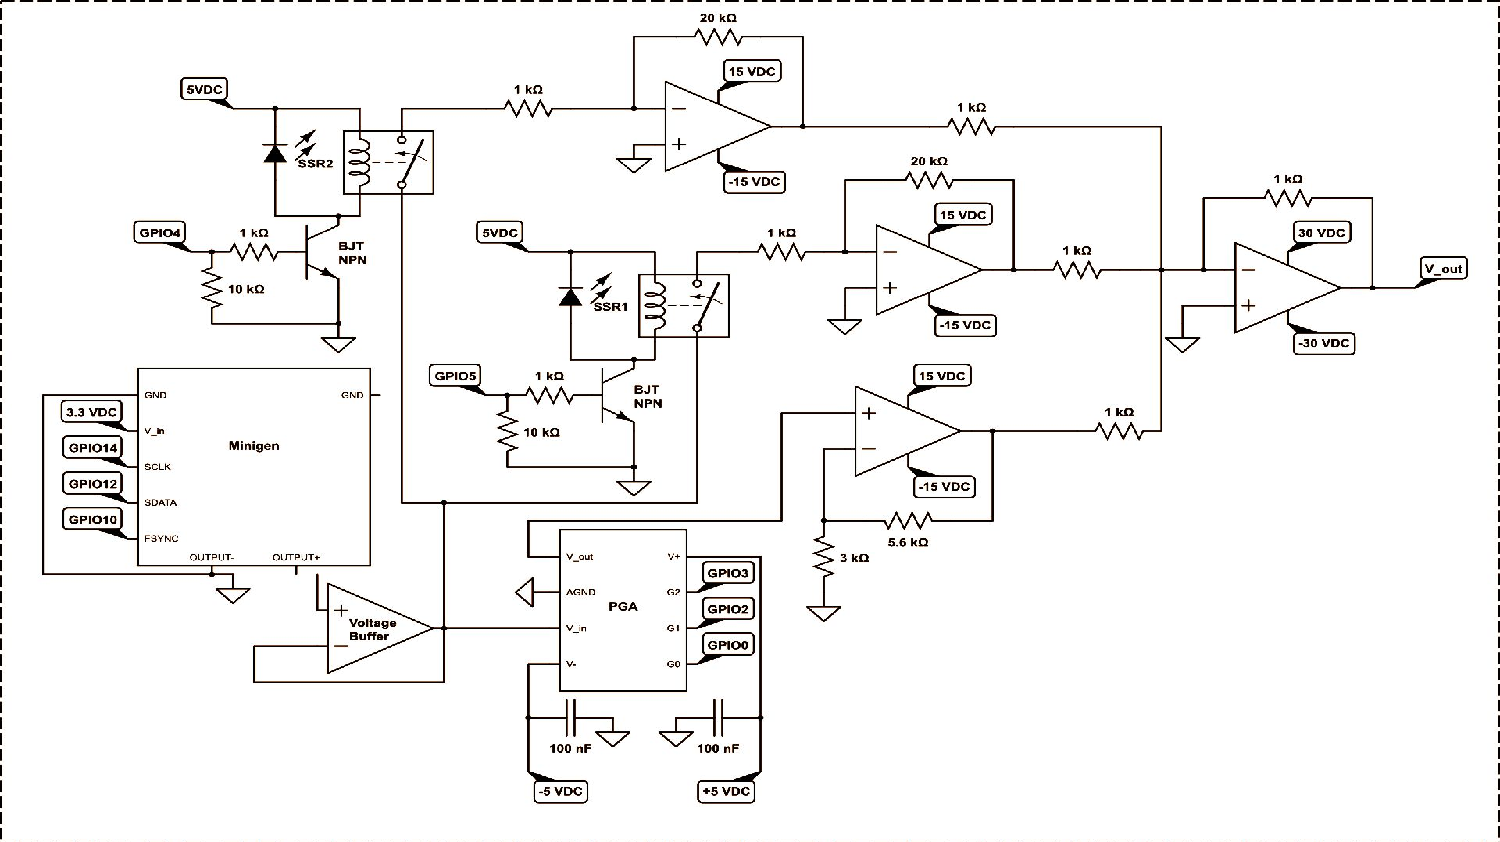
\includegraphics[width=0.8\textwidth,keepaspectratio]{ssr_implementation.pdf}
  \end{center}

  \begin{block}{Solid State Relay (SSR)}
  \begin{itemize}
    \item Uses LED and photo-resistor to allow current though
    \item Hoped to fix waveform distortion issues
  \end{itemize}
  \end{block}
\end{frame}

\subsection{Problems}

\begin{frame}{Problems}
  \begin{block}{Programmable Gain Amplifier(PGA)}
  \begin{itemize}
    \item Easy to destroy
    \item Functionally works well
  \end{itemize}
  \end{block}

  \begin{block}{Transistor Switch Circuit}
  \begin{itemize}
    \item BJT Leaks when logically off
  \end{itemize}
  \end{block}

  \begin{block}{Solid State Relay}
  \begin{itemize}
    \item Could not function at high enough frequency
    \item Even moderately high AC signals at input\\ cause output of 0
  \end{itemize}
  \end{block}
\end{frame}

% \begin{frame}{Problems and Setbacks}
%   \begin{itemize}
%     \item Lost a group member
%     \item BJT Switch
%     \item Control through GPIO pin
%     \item Current Leaks through when logically off
%     \item Relay
%     \item Operating Frequency not sufficient
%     \item Brandon
%     \item We have had to make quite a few adjustments from our original plan.
%     \item This is especially the case with our digital potentiometers.
%   \end{itemize}
% \end{frame}

\section{Final Design}

\begin{frame}{Overview}
\begin{block}{}
  \begin{itemize}
    \item Raspberry Pi controls integrated circuit components
    \item Minigen Function Generator
    \begin{itemize}
      \item SPI communications
      \item Produces frequency 10 Khz - 4 Mhz
    \end{itemize}
     \item Programmable Gain Amplifier(PGA)
    \begin{itemize}
      \item GPIO communications
      \item 8 voltage options (0-7)
    \end{itemize}
    \item Two-stage amplification
    \item Summing Amplifier
    \begin{itemize}
      \item Sums output from amplification stages
    \end{itemize}
  \end{itemize}
\end{block}
\end{frame}

\begin{frame}{Systems Diagram}
  \begin{center}
  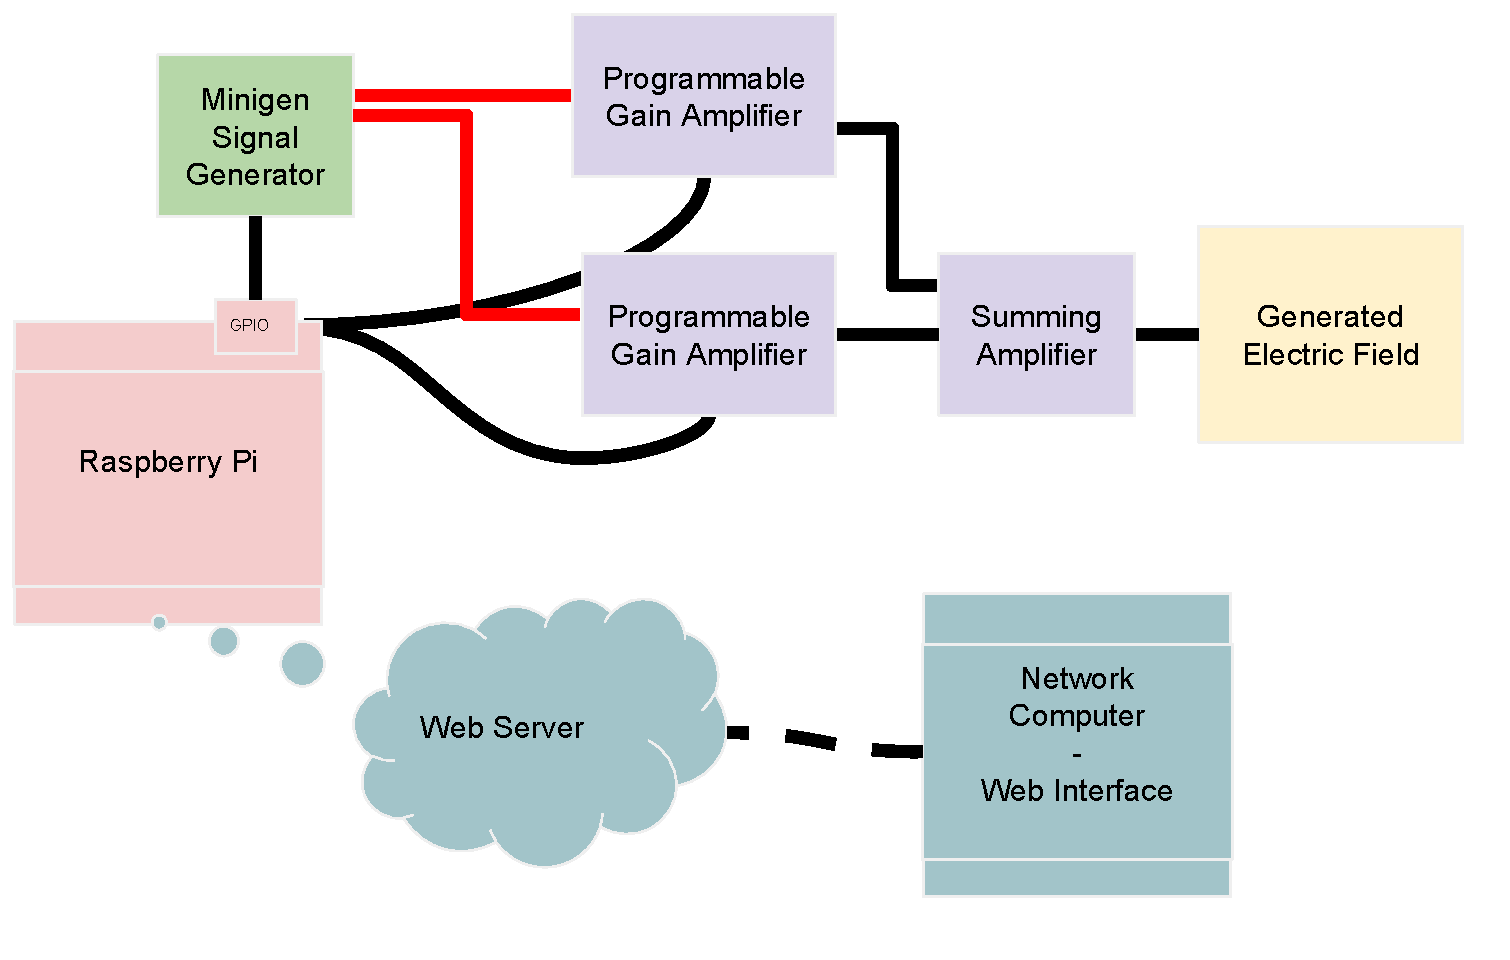
\includegraphics[width=1.0\textwidth,keepaspectratio]{block_diagram.pdf}
  \end{center}
\end{frame}

\subsection{Hardware Components}

\begin{frame}{Amplifier Circuit}
  %\begin{block}{}
  \begin{itemize}
    \item Two stages with PGA and constant gain amplifiers
    \begin{itemize}
      \item Upper stage constant amplifier Gain 7.5 
      \item Lower stage constant amplifier Gain 1.07
      \item PGA's both having variable gain
    \end{itemize}
    \item Summing amplifier
  \end{itemize}
  %\end{block}

  %\begin{center}
  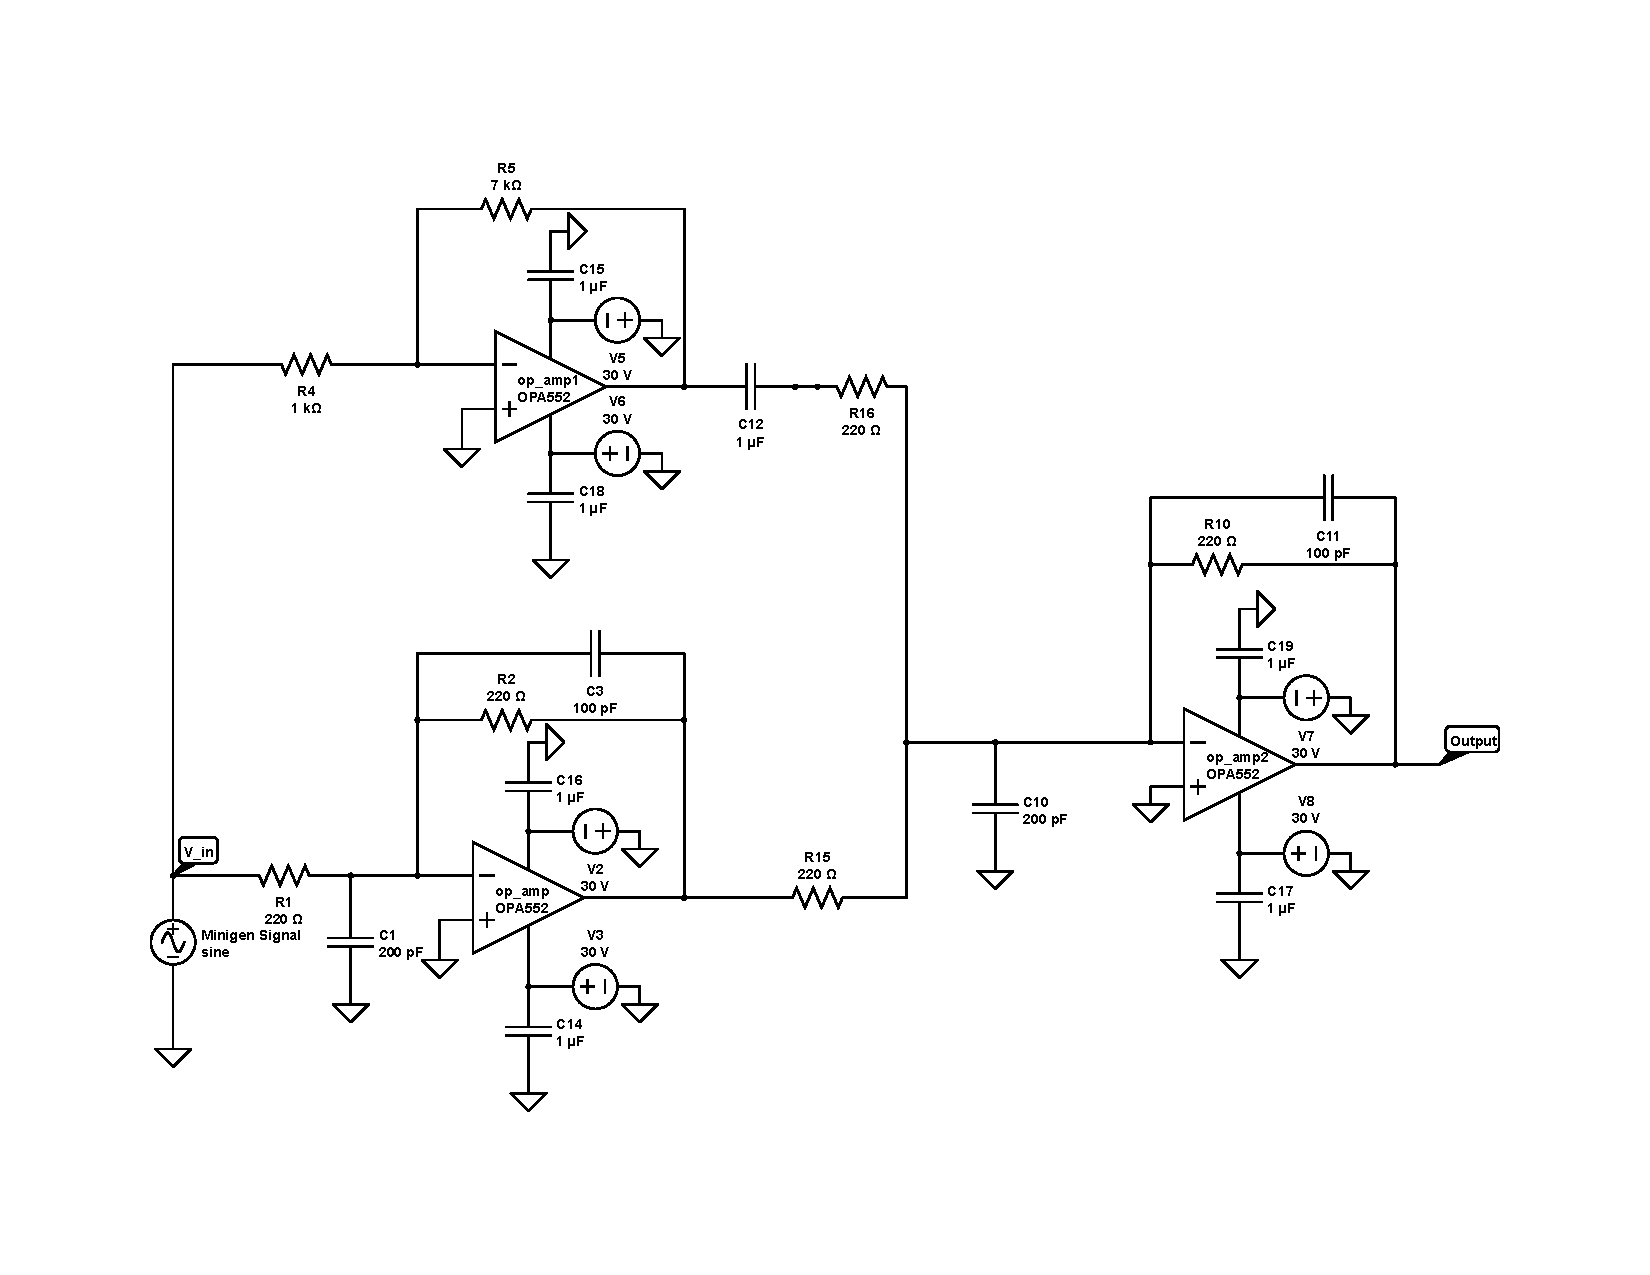
\includegraphics[width=1.0\textwidth,keepaspectratio]{circuit_diagram.pdf}
  %\end{center}
\end{frame}

% \begin{frame}{Computing Stage Gains}
%   \begin{itemize}
%     \item Hosted Locally
%   \end{itemize}
%     % voltage stage amplification computation
%     \begin{gather*}
%     A_1 = gain of stage 1 amp\\ 
%     A_2 = gain of stage 2 amp\\
%     A_{PGA} = max gain of PGA\\
%     V_{m1} = max voltage of stage 1\\
%     V_{m2} = max voltage of stage 2\\
%     V_{m1} + V_{m2} = 30V\\
%     V_{m1} = \frac{V_{m2}}{7}\\
%     V_{m1} + 7V_{m1} = 30V\\
%     8V_{m1} = 30V\\
%     V_{m1} = \frac{30V}{8}\\
%     V_{m1} = 3.75V\\
%     V_{m2} = 26.25V\\
%     A_{PGA} = 3.5V\\
%     A_1 = \frac{V_{m1}}{A_{PGA}} = \frac{V_{m1}}{3.5}\\
%     A_2 = \frac{V_{m2}}{A_{PGA}} = \frac{V_{m2}}{3.5}\\
%     A_1 = 1.07\frac{V}{V}\\
%     A_2 = 7.5\frac{V}{V}\\
%     \end{gather*}
% \end{frame}

\subsection{Software Components}

\begin{frame}{Web Interface}
\begin{multicols}{2}
  \begin{itemize}
    \item Hosted Locally
    \item Able to be seen on intranet
    \item Voltage and Frequency controls
    \item Provides Additional Functionality
  \end{itemize}

\newpage

%\begin{center}
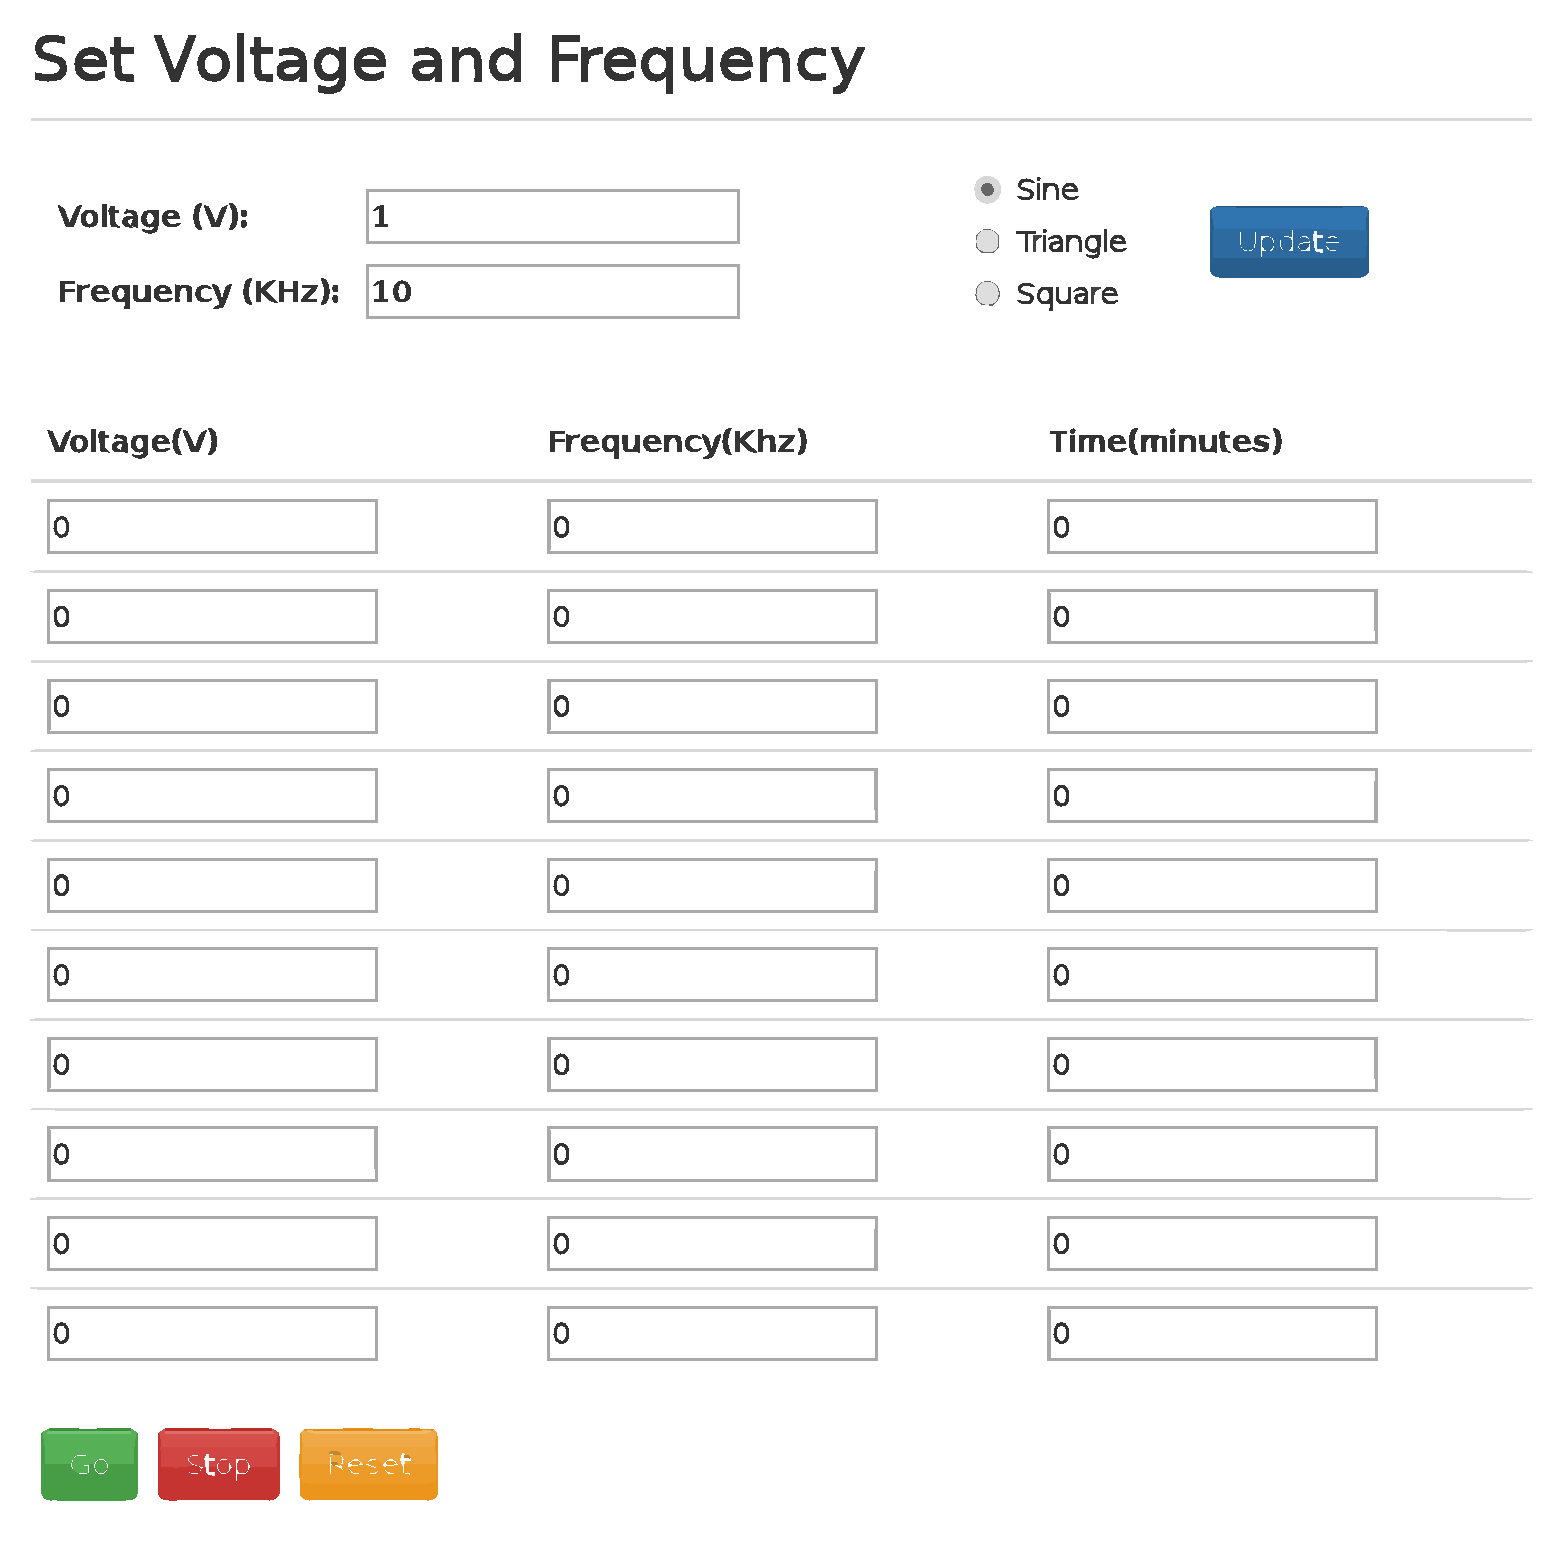
\includegraphics[width=0.5\textwidth,keepaspectratio]{web_interface.pdf}
%\end{center}

\end{multicols}
\end{frame}

% talk about how the web interface accomplishes its job
\begin{frame}{Software Components}
\begin{multicols}{2}

%\begin{center}
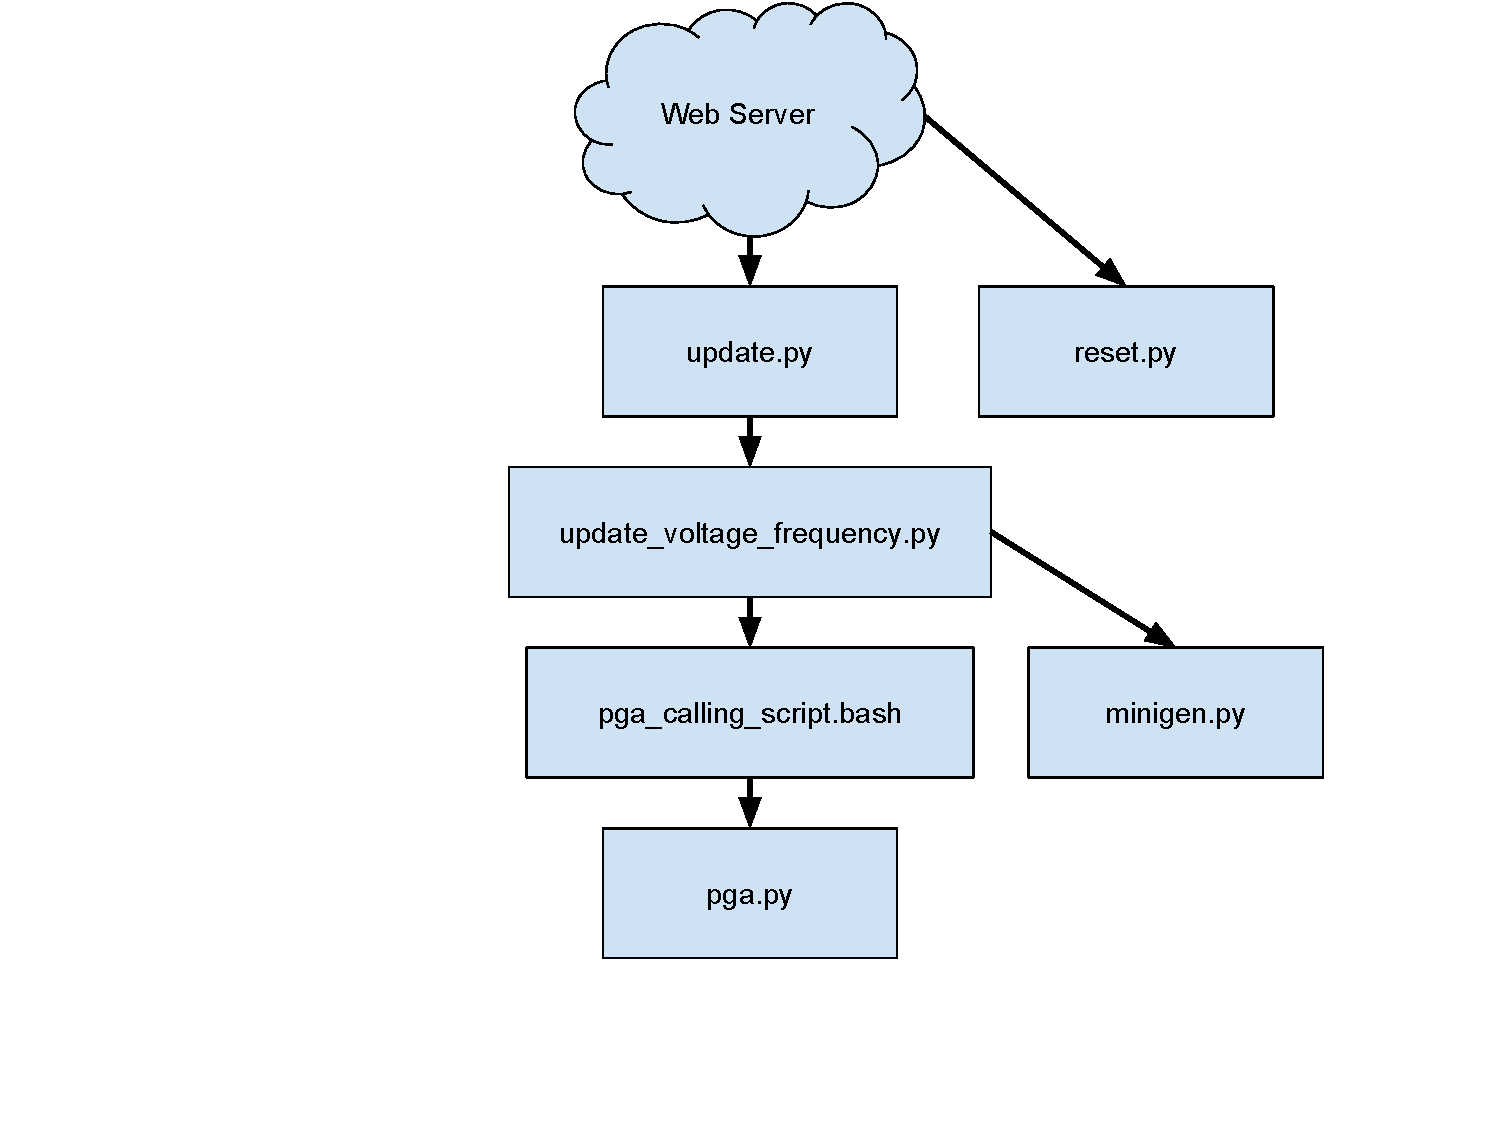
\includegraphics[width=.55\textwidth,keepaspectratio]{script_layout.pdf}
%\end{center}

\newpage

\begin{itemize}
  \item Script organization of the Raspberry Pi
  \item Delegation of Responsibility
  \item Scripts correspond to hardware components
\end{itemize}

\end{multicols}
\end{frame}

% discuss the final state of the project
\section{Current State}

% discuss issues with the current state
\begin{frame}{Current State}
  \begin{block}{Problems}
    \begin{enumerate}
      \item Minigen B23 Bug
      \item Current op-amps have insufficient Gain-Bandwidth Product
        \begin{enumerate}
        \item Insufficient frequency
        \item Insufficient voltage
        \end{enumerate}
      \item Current draw from Raspberry Pi
    \end{enumerate}
  \end{block}

  \begin{block}{Solutions}
    \begin{enumerate}
      \item Most probably a hardware issue
      \item An op-amp with necessary specifications exists, 598-1449-ND
      \item Ensure few additional components connected to the Pi
    \end{enumerate}
  \end{block}
\end{frame}

\begin{frame}{Cost}
\begin{block}{Itemized Expenditures}
  \begin{center}
    \begin{tabularx}{1.0\textwidth}{|X|X|X|}
        \hline

        \textbf{Item} &
        \textbf{Quantity} &
        \textbf{Price(\$)} \\
        \hline

        \textbf{Raspberry Pi 3 Kit} &
        \textbf{1} &
        \textbf{49.99} \\
        \hline

        \textbf{Micro SD card} &
        \textbf{1} &
        \textbf{9.99} \\
        \hline

        \textbf{Minigen Function Generator} &
        \textbf{1} &
        \textbf{29.95} \\
        \hline

        \textbf{Op Amps} &
        \textbf{3} &
        \textbf{4.41} \\
        \hline

        \textbf{PGA} &
        \textbf{2} &
        \textbf{8.00} \\
        \hline

        \textbf{Miscellaneous Components} &
        \textbf{-} &
        \textbf{10.5} \\
        \hline

        \hline
        \textbf{Total} &
        \textbf{-} &
        \textbf{104.84} \\

        \hline
    \end{tabularx}
  \end{center}
\end{block}
\end{frame}

\begin{frame}{Logistical Setbacks}
\begin{block}{}
  \begin{itemize}
    \item Lack of manpower
    \item Loss of a team member at semester break
    \item Point of contact left company
  \end{itemize}
\end{block}
\end{frame}

\begin{frame}{Deliverables}
\begin{block}{} 
  \begin{itemize}
    \item Raspberry Pi loaded with controlling code
    \item User manual
    \item Current circuit implementation
    \item PCB design
    \item Simulation files
  \end{itemize}
\end{block}

\begin{multicols}{4}

%\begin{center}
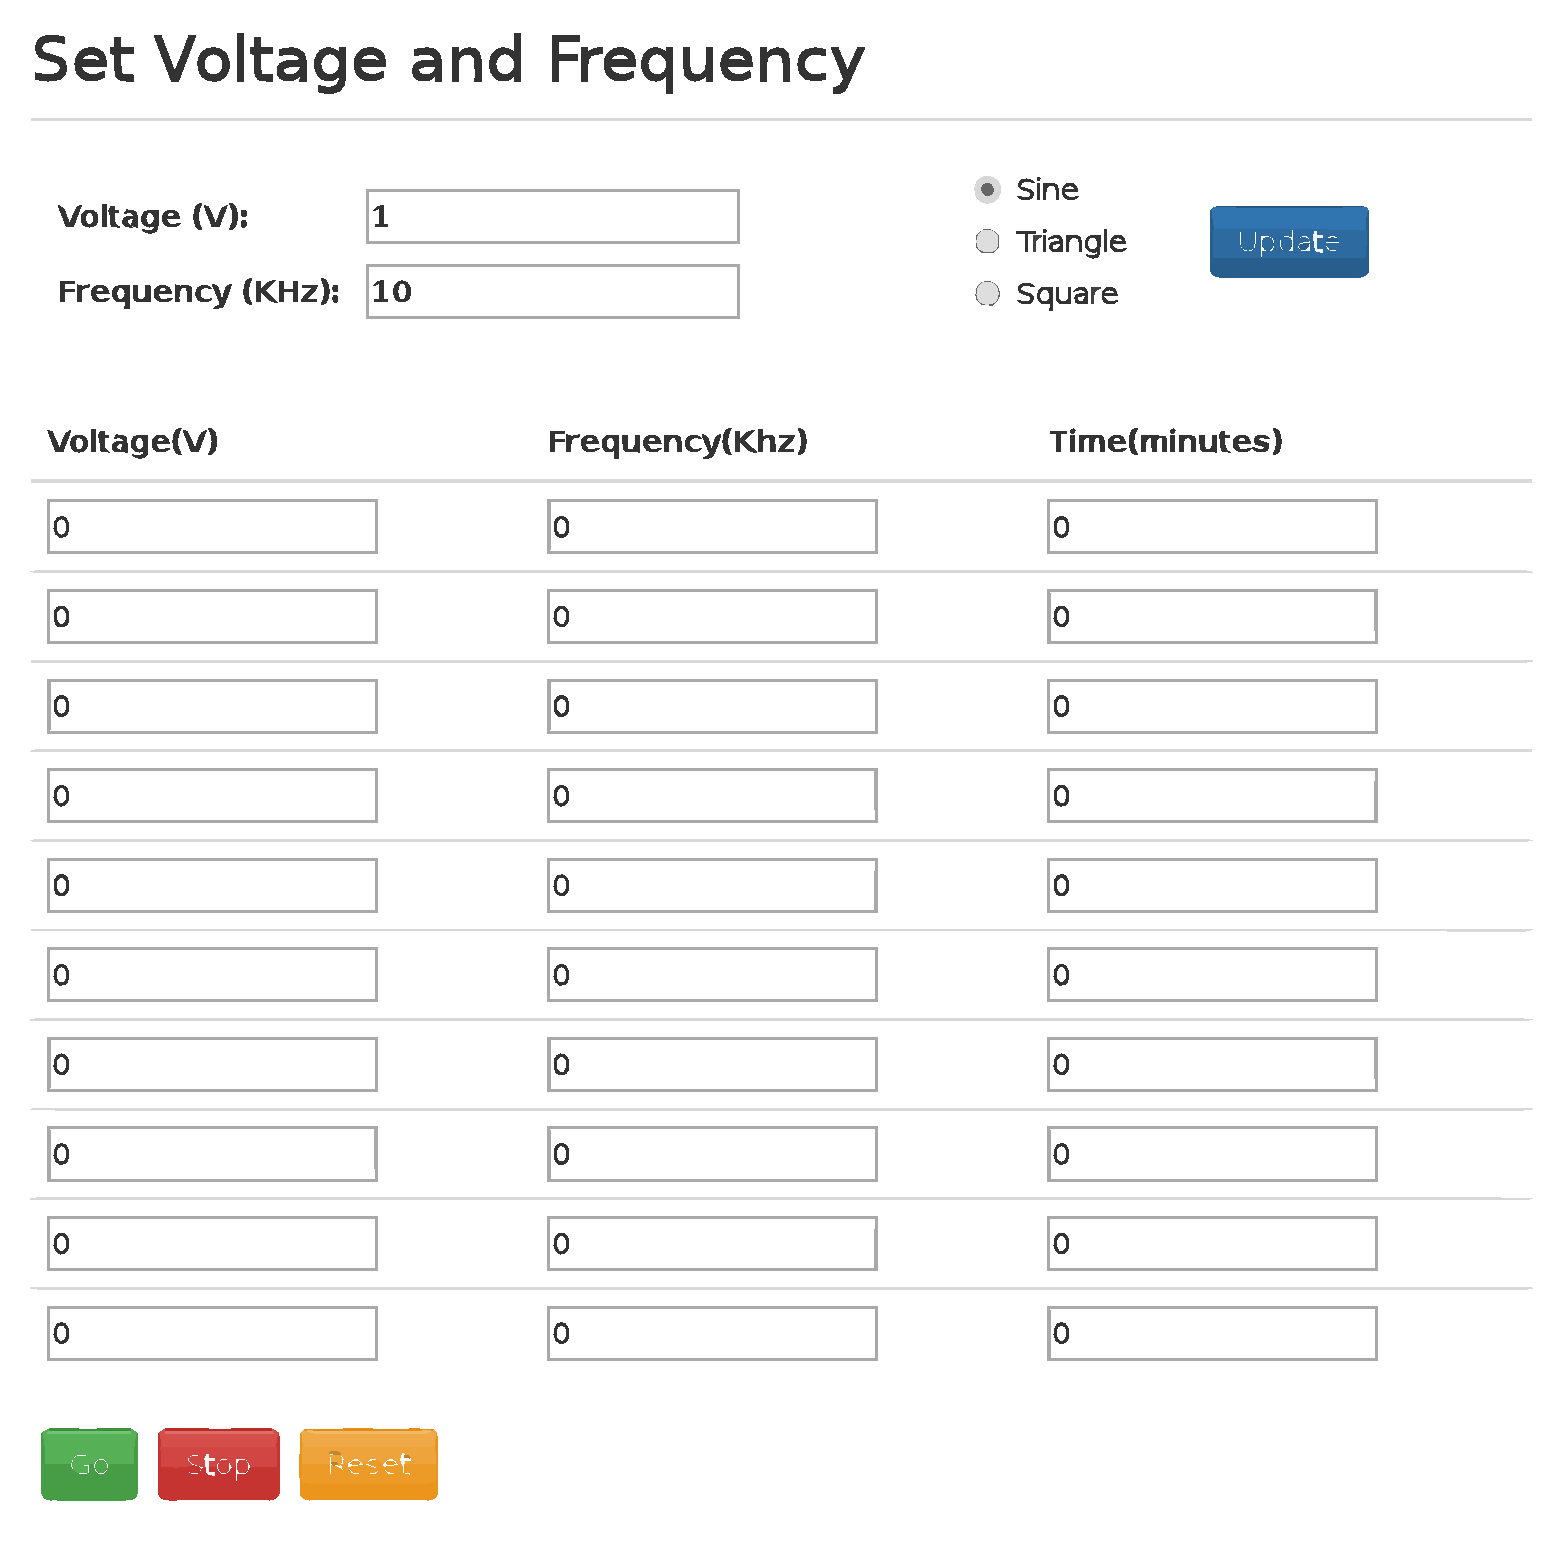
\includegraphics[width=.25\textwidth,keepaspectratio]{web_interface.pdf}
%\end{center}
%\begin{center}
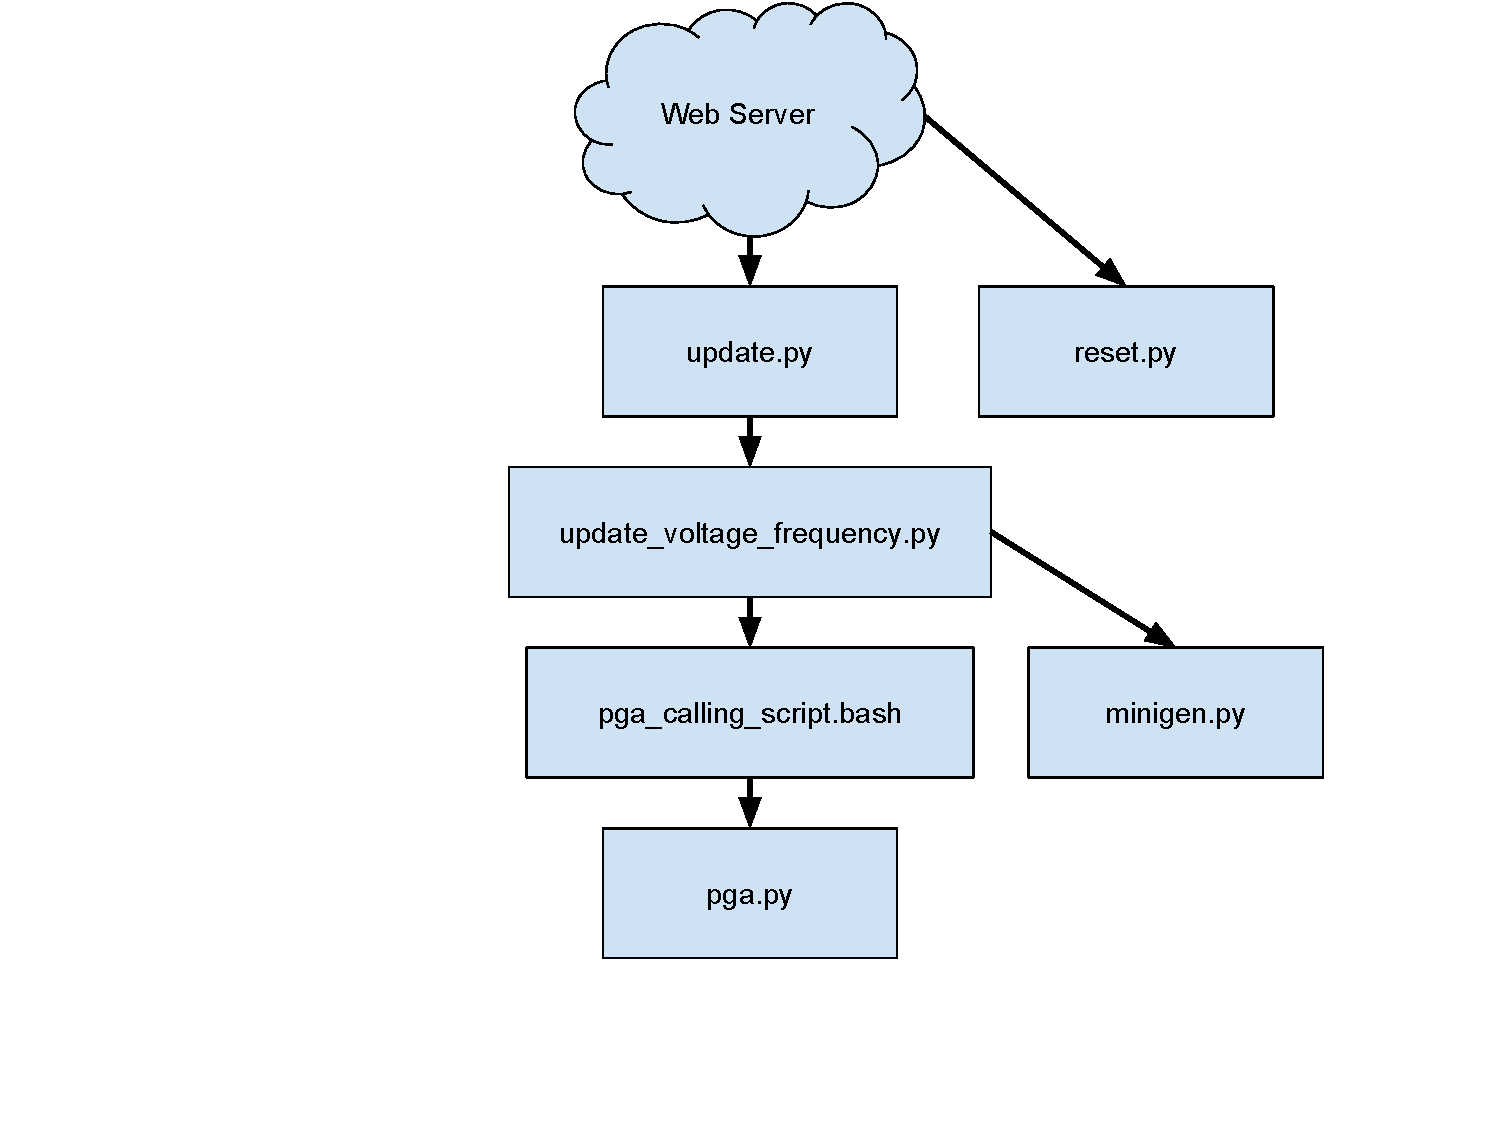
\includegraphics[width=.25\textwidth,keepaspectratio]{script_layout.pdf}
%\end{center}
%\begin{center}
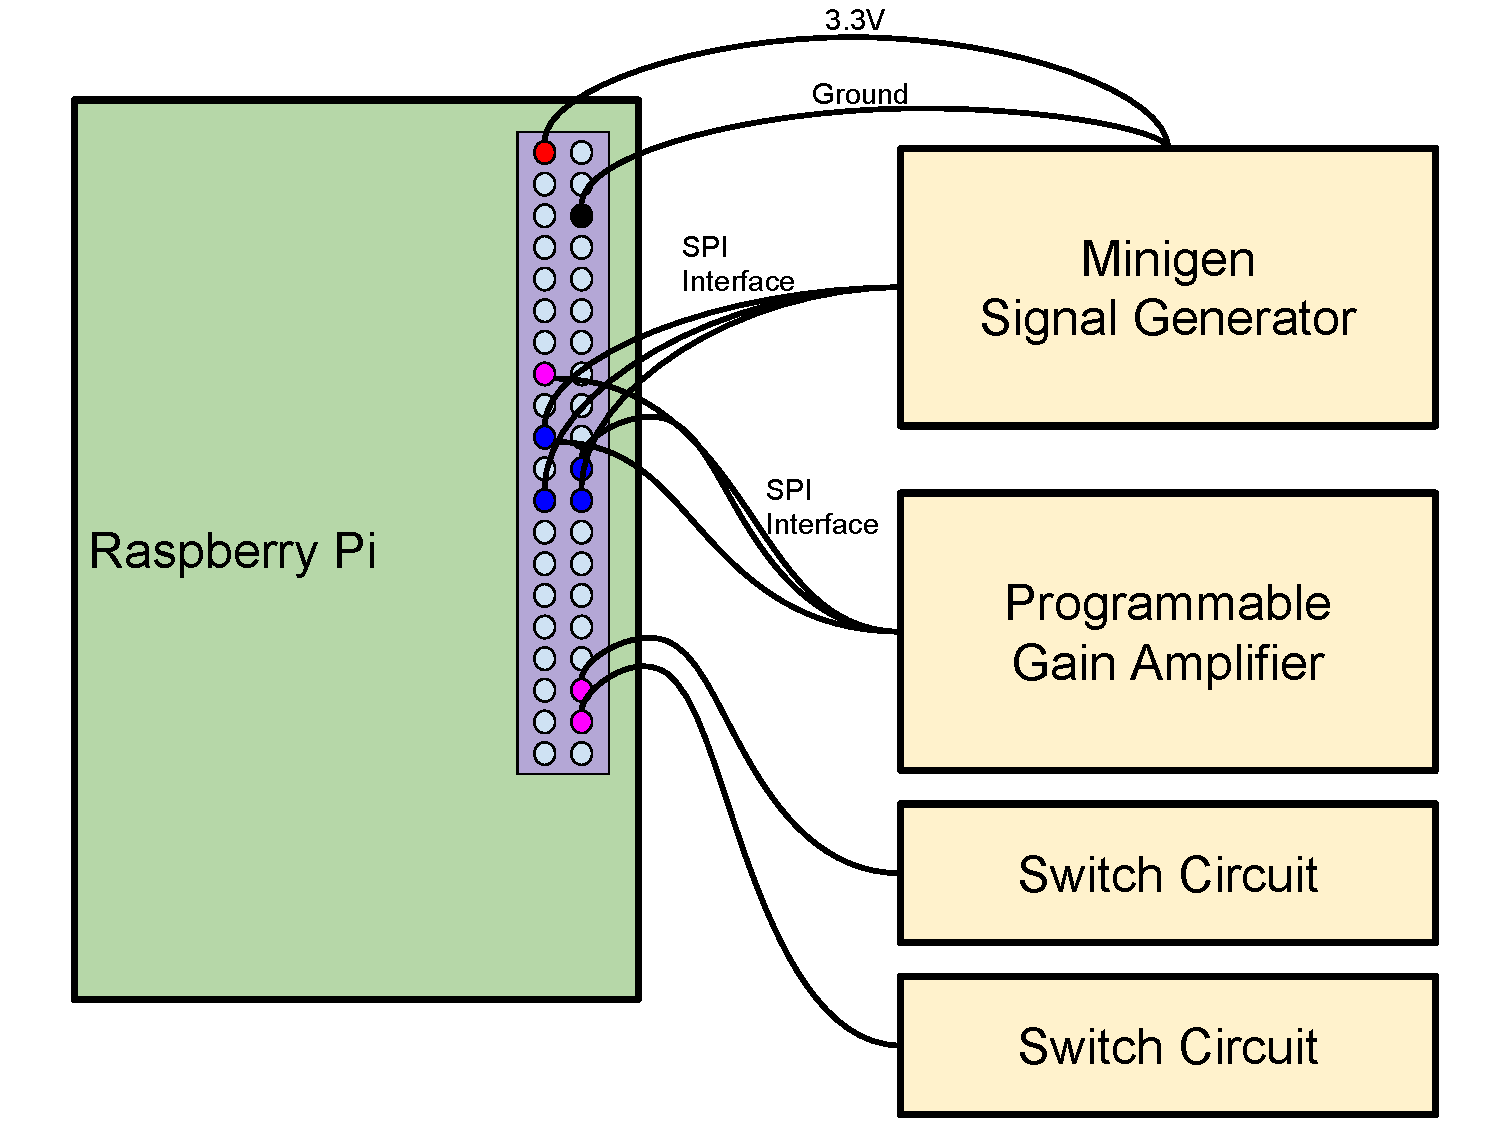
\includegraphics[width=.25\textwidth,keepaspectratio]{pi_connection.pdf}
%\end{center}
%\begin{center}
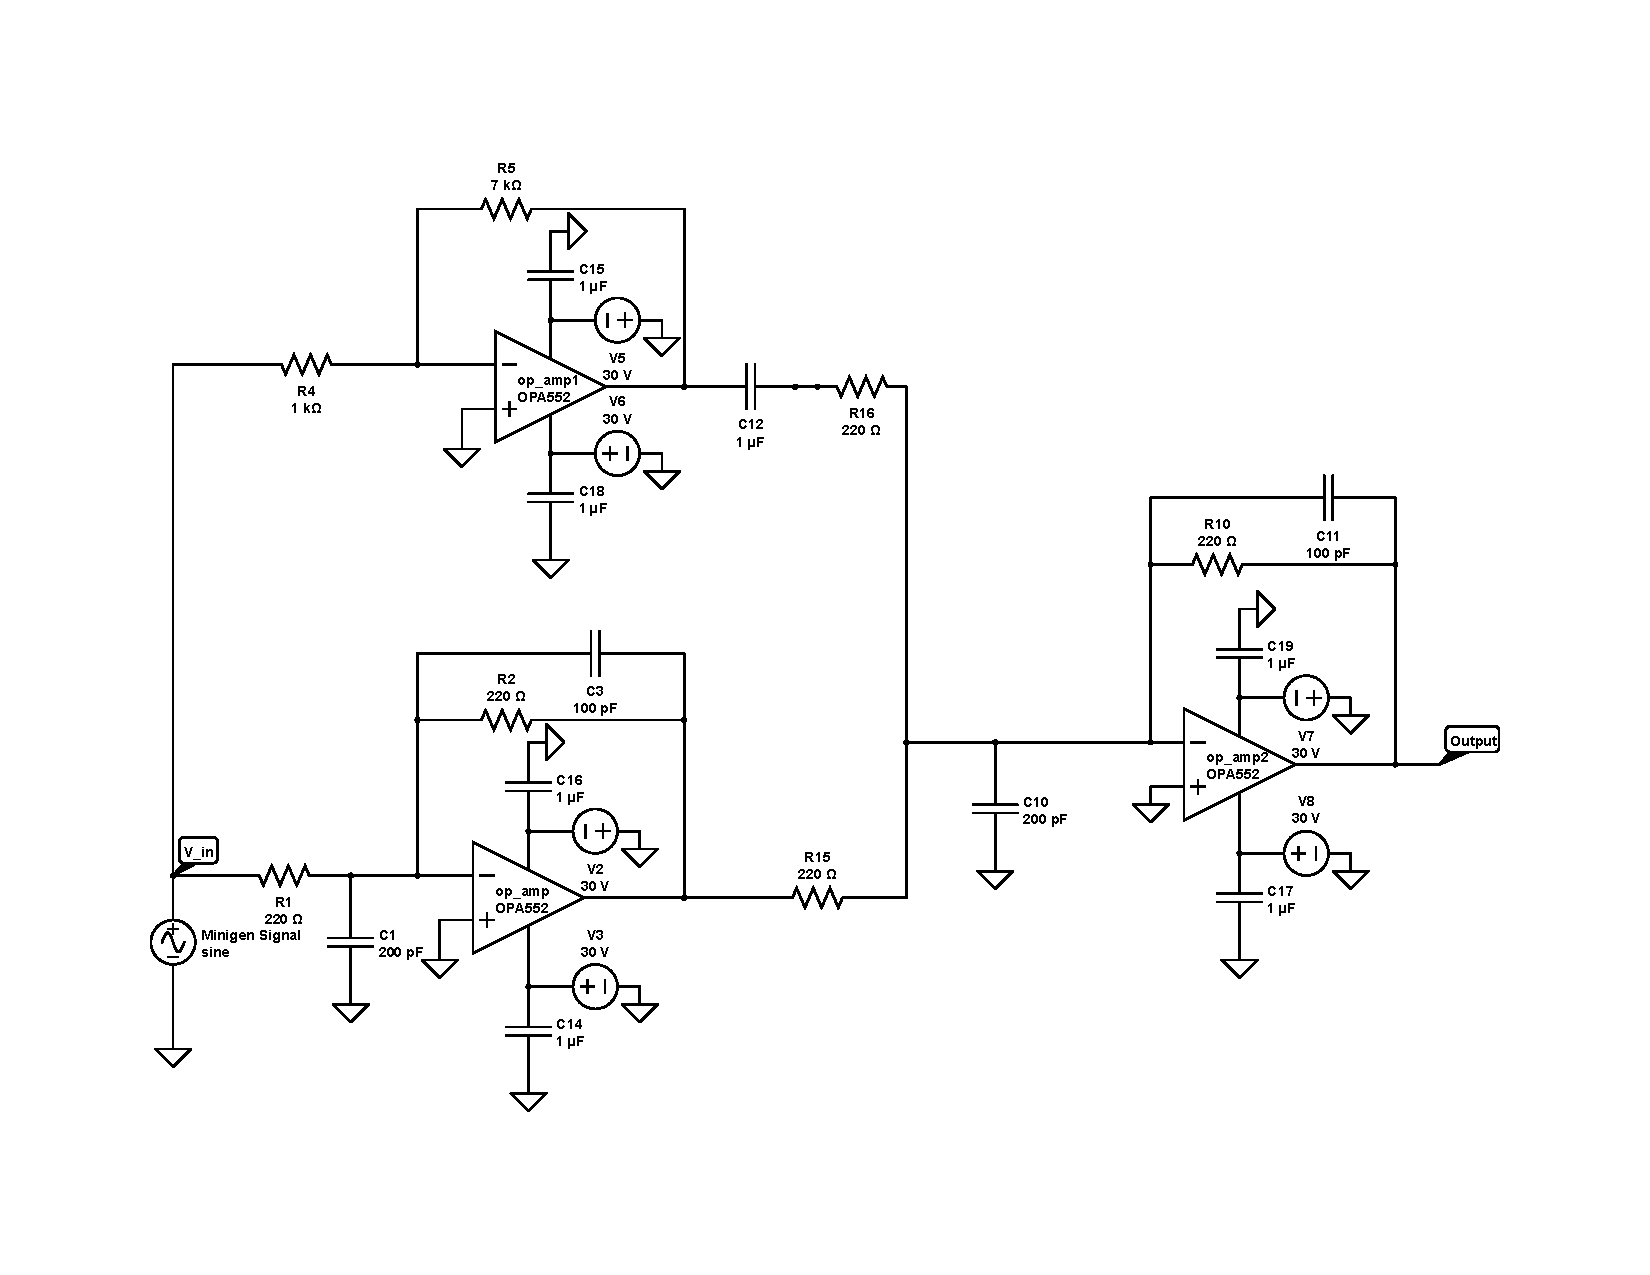
\includegraphics[width=.25\textwidth,keepaspectratio]{circuit_diagram.pdf}
%\end{center}

\end{multicols}
\end{frame}

\section{Questions}

\begin{frame}{Questions?}
\begin{block}{Discussion Points}
  \begin{itemize}
    \item Dielectrophoresis (DEP)
    \item Circuit Design
    \item Digital Potentiometer/ Operation Amplifier
    \item MOSFET/ Programmable Gain Amplifiers (PGA)
    \item Web Interface
    \item Final Documentation
  \end{itemize}
\end{block}
\end{frame}

%
% extra slides for answering questions
%

\begin{frame}{Work Breakdown}
\begin{block}{Items}
  \begin{itemize}
    \item Initial Planning
    \item Project Website
    \item Reports and documentation
    \item Circuit Design
    \item Web Server
    \item SOC Communications
    \item PCB Design
  \end{itemize}
\end{block}
\end{frame}

\end{document}